\chapter[Referencial Teórico]{REFERENCIAL TEÓRICO}
\label{ch:cap2}


Neste capítulo, são apresentados os principais conceitos utilizados neste trabalho, sendo eles: Redes Neurais Convolucionais com os seus hiperparâmetros e técnicas de compressão de dados com ênfase na no método da poda (pruning).

%\begin{equation}
%    a = \sum_{i=1}^n X_i * w_i
%\end{equation}

\section{Redes Neurais Convolucionais (CNN)} \label{secao1}
A rede neural convolucional é uma das classes de redes neurais utilizada para processamento e análise de imagens. Ela se diferencia dos outros tipos de redes neurais artificiais por possuir camadas convolucionais antes das camadas \textit{fully conected} e está presente em uma gama de aplicações como busca de imagens, recomendações de produtos, sistema de busca, reconhecimento facial entre outros. 

Assim como as ANNs, as redes neurais convolucionais possuem pesos que são alterados durante o processo de aprendizagem, a diferença é que nas camadas convolucionais, os pesos são organizados em \textit{kernels}, também chamados de filtros. Além das camadas convolucionais, é bastante comum a presença de camadas de \textit{pooling}, também conhecidas como camadas de agrupamento.

\subsection{Camada convolucional}
A camada convolucional da CNN consiste em um conjunto de filtros que serão operados por toda a imagem de entrada. Como o próprio nome diz, a operação realizada entre os filtros e a imagem de entrada é a chamada convolução, onde cada pixel da imagem de saída é o resultado da operação entre os elementos do filtro e regiões da imagem de entrada. Os hiperparâmetros desta camada incluem o tamanho do filtro, a quantidade de filtros, o \textit{stride} (passo) e se haverá, ou não, \textit{padding} (preenchimento). Se houver preenchimento, o tamanho da imagem de saída é igual ao de entrada. Porém, se não houver preenchimento, a imagem de saída será reduzida a depender do tamanho do \textit{kernel} e do \textit{stride} escolhido. Assim, o tamanho da imagem é dado por:

\begin{equation}
    L_s = L_e + k_s - 1 e
\end{equation}

\begin{equation}
    A_s = A_e + k_s - 1,
\end{equation}

Sendo $L_e$ e $A_e$ a lagura e altura da imagem de entrada, $L_s$ e $A_s$ a lagura e altura da imagem de saída e sendo $k_s$ o tamanho do \textit{kernel}. A Figura 1 mostra uma representação de como acontece o processo de convolução quando não há padding.

\begin{figure}[H]
    %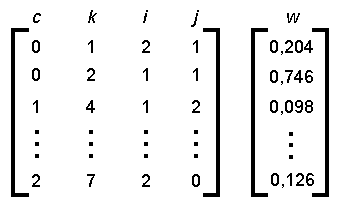
\includepdf[pages=-, width=6cm]{figuras/figx.pdf}
	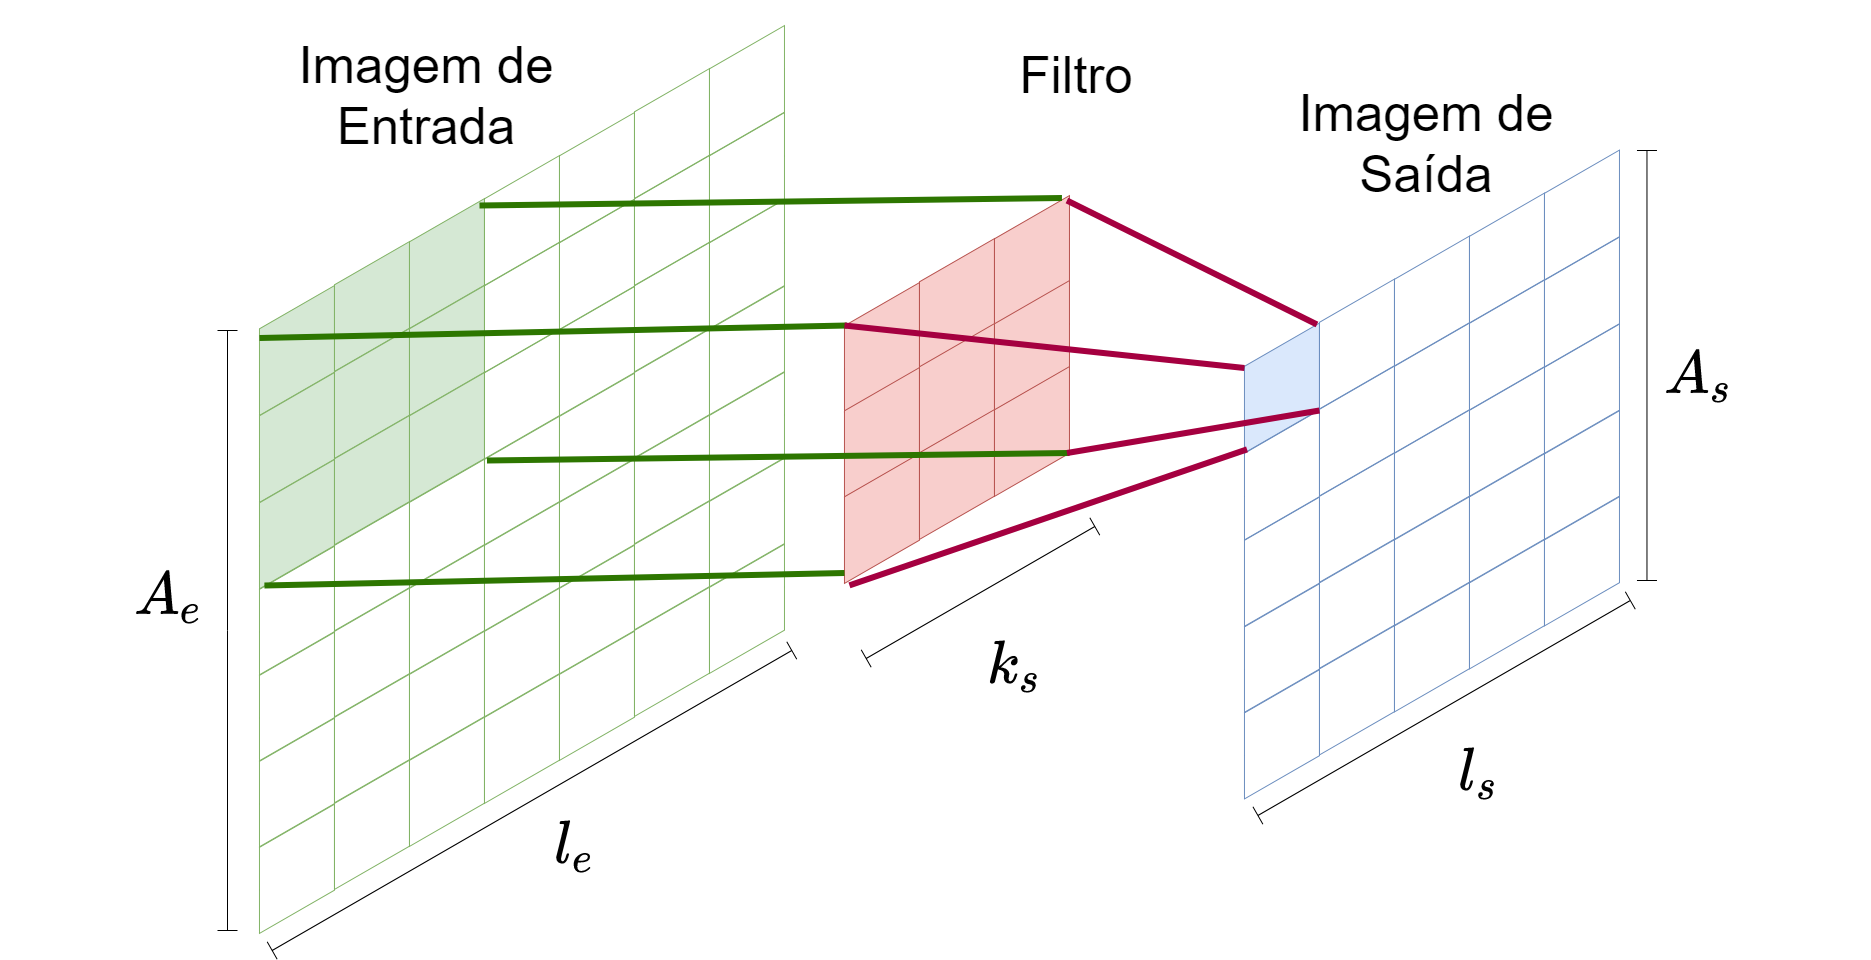
\includegraphics[width=0.45\textwidth, keepaspectratio=true]{figuras/CAP4/convv.png}
	\centering
	\caption[Operação de convolução]{Operação de convolução}
	\fonte{Elaborada pela autor.}
	%\label{fig:sharpe}
\end{figure}

\subsection{Camada de Agrupamento (\textit{Pooling})}
Na camada de agrupamento é realizado o processamento da imagem de entrada para redução da quantidade de parâmetros. Isso se faz selecionando, dentre um certo valor de parâmetros dentro da janela de \textit{pooling}, aquele que se adeque com o desejado. Normalmente, o agrupamento é feito a partir dos valores mais altos do grupo, através do \textit{max-polling}. Porém, o agrupamento pode ser realizado a partir do mínimo, do valor médio, entre outros.

Assim como a camada convolucional, é necessário escolher alguns hiperparâmetros para essa camada, como o tamanho da janela do agrupamento e o seu \textit{stride}. A Figura 2 apresenta a operação de \textit{max-pooling} para uma janela de agrupamento de tamanho 2 e \textit{stride} de 2, onde cada pixel da imagem de saída é o maior elemento dentro da janela de 4 elementos.

\begin{figure}[H]
    %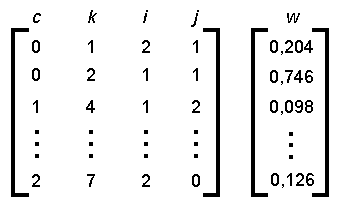
\includepdf[pages=-, width=6cm]{figuras/figx.pdf}
	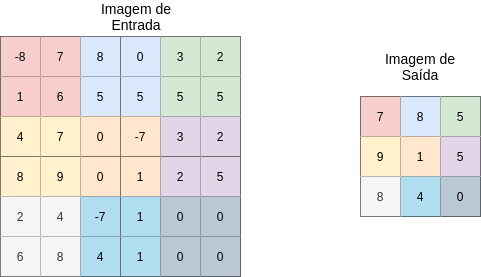
\includegraphics[width=0.5\textwidth, keepaspectratio=true]{figuras/poolig.png}
	\centering
	\caption[Operação de \textit{max-pooling}]{Operação de \textit{max-pooling}}
	\fonte{Elaborada pela autor.}
	%\label{fig:sharpe}
\end{figure}

\subsection{Camada de \textit{flattening}}

A Figura 3 ilustra o processo de flattening, que é responsável por realiza uma transformação na matriz da imagem, alterando seu formato para um vetor. Por exemplo, se a entrada da camada de \textit{flattening} for uma matriz de 32x32x3, a saída será um vetor de 3072 posições.

\begin{figure}[H]
    %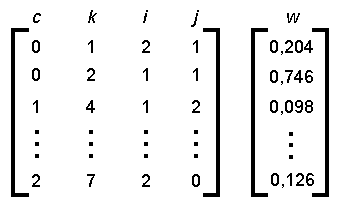
\includepdf[pages=-, width=6cm]{figuras/figx.pdf}
	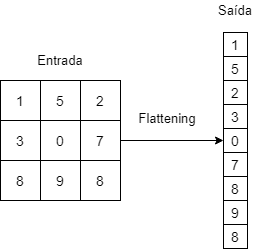
\includegraphics[width=0.22\textwidth, keepaspectratio=true]{figuras/flatten (1).png}
	\centering
	\caption[Operação de \textit{flattening}]{Operação de \textit{flattening}}
	\fonte{Elaborada pela autor.}
	%\label{fig:sharpe}
\end{figure}

\subsection{Camada \textit{fully-connected} (totalmente conectada)}
A camada totalmente conectada é a camada mais utilizada em aplicações de redes neurais. Ela se forma a partir da conexão de todos os neurônios de entrada e saída por pesos. Como hiperparâmetro, pode-se definir a quantidade de parâmetros a serem utilizados. A Figura 4 apresenta um modelo convencional de camadas totalmente conectadas.

\begin{figure}[H]
    %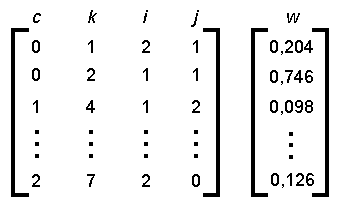
\includepdf[pages=-, width=6cm]{figuras/figx.pdf}
	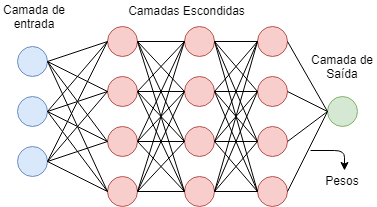
\includegraphics[width=0.35\textwidth, keepaspectratio=true]{figuras/rede.png}
	\centering
	\caption[Estrutura e operações da camada \textit{fully-connected}]{Estrutura e operações da camada \textit{fully-connected}}
	\fonte{Elaborada pela autor.}
	%\label{fig:sharpe}
\end{figure}

A Figura 5 ilustra as operações realizadas entre entre os neurônios e os pesos, onde $X_n$ é o valor armazenado no \textit{n}-ésimo neurônio e $w_n$ é o peso que conecta o neurônio da camada anterior com o neurônio da camada atual.

\begin{figure}[H]
    %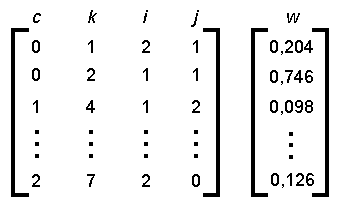
\includepdf[pages=-, width=6cm]{figuras/figx.pdf}
	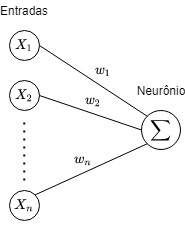
\includegraphics[width=0.2\textwidth, keepaspectratio=true]{figuras/rna.png}
	\centering
	\caption[Operações realizadas na camada \textit{fully-connected}]{Operações realizadas na camada \textit{fully-connected}}
	\fonte{Elaborada pela autor.}
	%\label{fig:sharpe}
\end{figure}

\subsection{Funções de ativação}
A aplicação da função de ativação pode ser utilizada em qualquer camada da rede. Ela é a transformação não linear que é feita ao longo da entrada. A saída desta função é enviada para a próxima camada. Uma rede neural sem função de ativação torna-se apenas um modelo linear, sendo que a maioria dos problemas complexos resolvidos por redes neurais são não-lineares.

Existem diversas funções de ativação diferentes. Para este trabalho foram utilizadas apenas duas: a ReLU e a softmax. A função ReLU é definida na Equação 2.3, onde $y$ é a saída da função que retorna o valor máximo entre 0 e o valor de $x$, que é o parâmetro sendo analisado. A Figura 6 mostra o gráfico dessa função.

\begin{equation}
    y = max(0,x)
\end{equation}

\begin{figure}[H]
    %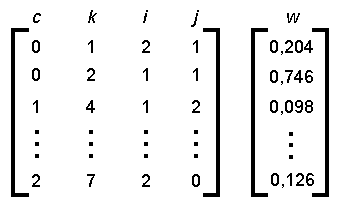
\includepdf[pages=-, width=6cm]{figuras/figx.pdf}
	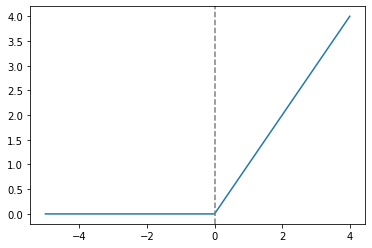
\includegraphics[width=0.4\textwidth, keepaspectratio=true]{figuras/relu.png}
	\centering
	\caption[Função de ativação ReLU]{Função de ativação ReLU}
	\fonte{Elaborada pela autor.}
	%\label{fig:sharpe}
\end{figure}

A função de ativação softmax, também conhecida como softargmax ou função exponencial normalizada, é uma função que recebe um vetor com \textit{z} números reais e o normaliza em uma distribuição probabilistica para os \textit{z} valores. Essa função é normalmente utilizada na camada de saída para que seja representada a probabilidade da imagem em análise pertencer a cada uma das classes. Essa função é definida na Equação 2.4, onde $z_i$ é o \textit{i}-ésimo termo do vetor z e $z_j$ é o \textit{j}-ésimo termo do mesmo vetor. Essa função é representada graficamente na Figura 7.

\begin{equation}
    S(z_i) = \frac{e^{z_i}}{\sum_{j=1}^k e^{z_j}}
\end{equation}

\begin{figure}[H]
    %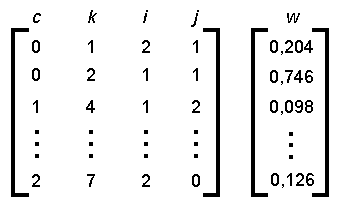
\includepdf[pages=-, width=6cm]{figuras/figx.pdf}
	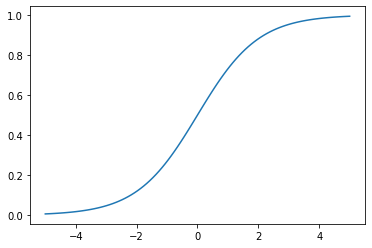
\includegraphics[width=0.4\textwidth, keepaspectratio=true]{figuras/softmax.png}
	\centering
	\caption[Função de ativação softmax]{Função de ativação softmax}
	\fonte{Elaborada pela autor.}
	%\label{fig:sharpe}
\end{figure}

\section{Técnicas de compressão de modelo} \label{secao1}
As estratégias para aceleração de inferência podem ser classificadas em baseadas em algoritmos e baseada em sistemas. Abordagens de aceleração baseadas em algorítmos incluem: processamento paralelo, compressão de modelo, exploração de esparsidade e redução de modelo por aproximação. Já as abordagens de aceleração baseadas em sistemas abrangem sistemas de memória de alta largura de banda para minimizar o tempo de acesso à memória, aceleradores de hardware, sistemas de computação distribuída e otimizações de compilador, como eliminação de expressão comum. A estratégia baseada em algoritmos usando compresão, foco deste trabalho, é uma forma comum na redução do número de operações nas redes neurais profundas.


\subsection{Exploração de esparsidade}

Uma matriz é dita esparsa quando a maior parte de seus elementos são zeros. A exploração da esparsidade pode estar presente em multiplos níveis: \textit{bit}, valor, canal, filtro, bloco entre outros. O valor da esparsidade de certa camada, ou modelo, é encontrado a partir da Equação 2.5, onde $n_{zeros}$ representa a quantidade de zeros e $n_{pesos}$ representa a quantidade de pesos.

\begin{equation}
    esparsidade = \frac{n_{zeros}}{n_{pesos}}*100%
\end{equation}

A esparsidade também pode ser computada a partir da contagem de elementos com magnitude muito próximas a zero, ou não significativos. A Tabela 1 apresenta um exemplo da esparsidade de uma rede neural com 65536 parâmetos, onde $W_k$ representa o limite que define a magnitude dos pesos que são considerados insignificantes para o modelo a coluna de Quantidade de pesos mostra quantos pesos são removidos para cada limite de $W_k$ e a teceira coluna mostra as esparsidades do modelo.

\begin{table}[H]
    \centering
    \begin{tabular}{ |p{3cm}|p{3cm}|p{3cm}|  }
 %\hline
 %\multicolumn{2}{|c|}{Estrutura da rede utilizada} \\
 \hline
 Mag. do peso&Qtd. de pesos&Esparsidade \\
 \hline
    $W_k$ < 0.01            &6438    &   9,82\%\\
    $W_k$ < 0.001           &3220    &   4,91\%\\
    $W_k$ < 0.0001          &1924    &   2,94\%\\
 \hline
 \multicolumn{3}{|c|}{Rede neural com 65536 pesos} \\
 \hline
\end{tabular}
    \caption{Esparsidade para pesos com diferentes magnitudes}
    \label{tab:my_label}
\end{table}

\subsection{Compressão de modelo por poda}
Atualmente, diferentes técnicas de compressão de modelo são utilizados, como quantização da rede, poda e ajuste fino de modelos pré-treinados. A compressão de modelo também pode ser realizada a partir da quantização seguida da poda ou da poda seguida da quantização. 

A otimização utilizando a técnica de poda, objeto deste trabalho, consiste na remoção de pesos insignificantes do modelo a partir de um certo \textit{threshold} (limiar). A definição deste limiar expressa o quão agressiva será a poda no modelo, sendo que a remoção de muitos pesos pode afeter significativamente a acurácia da rede. A remoção desses pesos faz com que a quantidade de operações realizadas durante a inferêmcia da rede seja menor que a do modelo não comprimido. A figura 8 mostra como acontece a remoção dos pesos do modelo.

\begin{figure}[H]
    %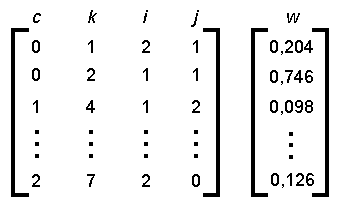
\includepdf[pages=-, width=6cm]{figuras/figx.pdf}
	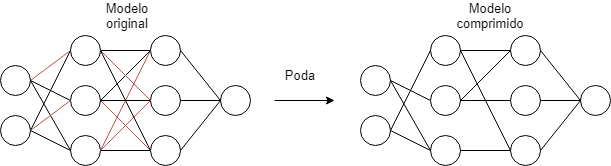
\includegraphics[width=0.6\textwidth, keepaspectratio=true]{figuras/poda.png}
	\centering
	\caption[Representação da técnica de poda]{Representação da técnica de poda}
	\fonte{Elaborada pela autor.}
	%\label{fig:sharpe}
\end{figure}

A remoção dos pesos ocorre durante o loop de aprendizagem do modelo. As técnicas mais convencionais realizam a remoção dos pesos apenas no primeiro \textit{batch} de cada época, outras realizam o mesmo processo apenas no final de cada época. O \textit{loop} de aprendizado de \textit{prune-aware} pode ser visualizado na Figura 9. Onde $Y(n)$ é a classe predita do modelo para a entrada $X_n$, $Yref(n)$ é a classe real da entrada, $E(n)$ é o erro obtido pela diferença entre a saída predita e a saída real, $G(n)$ é a aplicação do gradiente de decida levando em consideração tanto o erro quanto os pesos removidos. $W(n)$ é o \textit{n}-ésimo peso, $Z^{-1}$ é um atraso e $C(n)$ é o resulado do peso que sofreu a poda. Para o controle do momento que deverá haver a poda, existe uma chave de controle de época que fecha ou abre o caminho com a remoção do peso quando desejado.


\begin{figure}[!h]
    %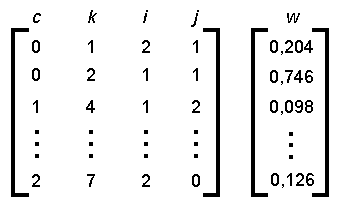
\includepdf[pages=-, width=6cm]{figuras/figx.pdf}
	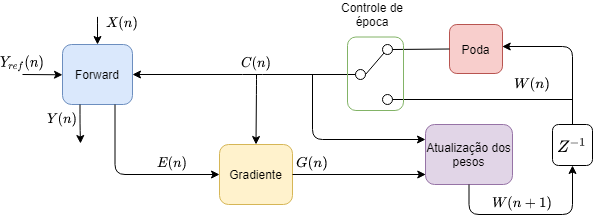
\includegraphics[width=0.7\textwidth, keepaspectratio=true]{figuras/prune_normal (1).png}
	\centering
	\caption[loop de aprendizado de \textit{prune-aware} convencional]{loop de aprendizado de \textit{prune-aware} convencional}
	\fonte{Elaborada pela autor.}
	%\label{fig:sharpe}
\end{figure}


%\section[\textit{Seção}]{\textit{Seção}}
%\lipsum[1-2]

%Itens em latex:
%\begin{itemize}
%	\item texto 1;
%	\item texto 2;
%	\item texto 3;
%\end{itemize}

%\lipsum[2-3]

%\subsection{Subseção}

%\lipsum[2-4]